\section{Etape B : vérifications contextuelles et décorations}

Cette étape permet de vérifier la correction contextuelle du programme d'entrée ainsi que de rajouter à l'arbre abstrait les informations nécessaires (décorations) pour l'étape suivante (génération de code).


  \begin{center}
    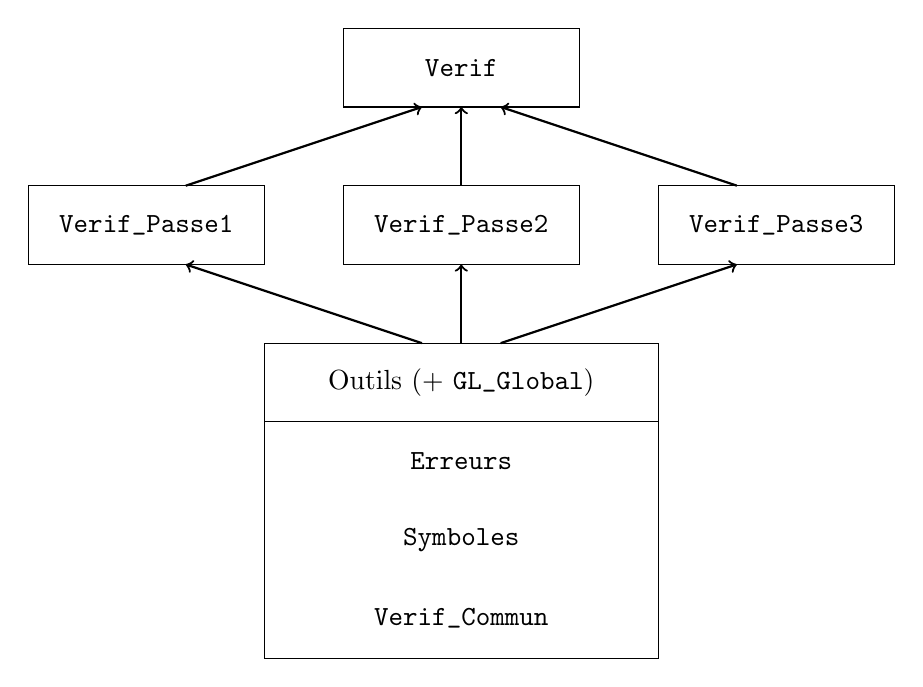
\begin{tikzpicture}
      \draw (3,0) rectangle (8, 4);
      \draw (5.5,3.5) node {Outils (+ \verb!GL_Global!)};
      \draw (3,3) -- (8,3);
      \draw (5.5,2.5) node {\verb!Erreurs!};
      \draw (5.5,1.5) node {\verb!Symboles!};
      \draw (5.5,0.5) node {\verb!Verif_Commun!};

      \draw (0,5) rectangle (3,6);
      \draw (1.5,5.5) node {\verb!Verif_Passe1!};
      \draw[->,thick] (5,4) -- (2,5);
      \draw[->,thick] (2,6) -- (5,7);

      \draw (4,5) rectangle (7,6);
      \draw (5.5,5.5) node {\verb!Verif_Passe2!};
      \draw[->,thick] (5.5,4) -- (5.5,5);
      \draw[->,thick] (5.5,6) -- (5.5,7);

      \draw (8,5) rectangle (11,6);
      \draw (9.5,5.5) node {\verb!Verif_Passe3!};
      \draw[->,thick] (6,4) -- (9,5);
      \draw[->,thick] (9,6) -- (6,7);

      \draw (4,7) rectangle (7,8);
      \draw (5.5,7.5) node {\verb!Verif!};
    \end{tikzpicture}
  \end{center}



\subsection{Implémentation en trois passes : \texttt{Verif\_Passe[123]}}

La vérification contextuelle et la décoration de l'arbre abstrait sont réalisées suivant 3 parcours de l'arbre abstrait généré en étape A. \\
Les passes (ou parcours) sont implémentées dans des paquetages distincts, qui définissent un ensemble de procédures de parcours de l'arbre abstrait, ainsi qu'un unique point d'entrée : \verb!Verifier_Decorer_[123]!.
Ces passes remplissent des rôles bien définis suivant la grammaire attribuée du langage Deca.
\begin{itemize}
\item Paquetage \verb!Verif_passe1.adb! : \\Ce paquetage vérifie la validité du nom des classes et la hiérarchie entre elles (extends). On génère un environnement contenant l'environnement prédéfini des types ainsi que ceux des classes définies dans le programme Deca. La décoration des classes sera faite durant la première passe.
\item Paquetage \verb!Verif_passe2.adb! : \\Ce paquetage vérifie la validité des déclarations des champs et la signature des méthodes des classes. On construit un environnement spécifique à chaque classe. La décoration des champs et des méthodes est réalisée durant cette passe, dans laquelle on trouvera notamment son numéro. Enfin on met aussi à jour les informations des classes par son nombre de champs et son nombre de méthodes.
\item Paquetage \verb!Verif_passe3.adb! : \\Ce paquetage vérifie les initialisations et le corps des méthodes. On vérifie aussi le programme principal. Cette passe s'appuie sur les différents environnements crées dans les passes précédentes pour livrer son résultat. On décore aussi le noeud "Retour", les noeuds "Ident" et les noeuds "EXP".
\end{itemize}

L'organisation de chacun de ces trois paquetages est similaire et calquée autant que possible sur la grammaire attribuée correspondante. Dans la majorité des cas,
les procédures sont nommées \verb!Verif_<Nom>!, où ``nom'' est un non-terminal de la grammaire attribuée.


\subsection{Packages "Outils"}

\subsubsection{Opérations communes aux trois passes: \texttt{Verif\_Commun}}
 Le paquetage \verb!Verif_Commun! centralise les diverses opérations qui sont communes aux trois passes, on distingue:
\begin{itemize}
\item Les opérations sur les environnements (union disjointe)
\item Un test de comparaison des signatures des méthodes
\item Les tests sur la compatibilité des types pour la conversion et l'affectation
\item Les tests sur la compatibilité des types pour les opérateurs
\item L'implémentation des règles communes aux 3 grammaires
\end{itemize}

\subsubsection{Environnements prédéfinis : \texttt{Symboles}}

On définit les environnements prédéfinis \verb!Env_Types_Predef! et \verb!Env_Exp_Object! dans le paquetage \verb!Symboles!. \\
L'environnement prédéfini \verb!Env_Types_Predef! contient la définition des types de bases (int, float, boolean) ainsi que celle de void et de la classe Object.
L'environnement prédéfini \verb!Env_Exp_Object! contient l'environnement de la classe Object, à savoir la méthode equals.
Le paquetage fournit également la procédure chargée de rechercher une définition dans un environnement donné. Concrètement, il s'agit simplement de parcourir le chainage des \verb!Table_Defn! jusqu'à trouver l'entrée cherchée (si elle existe).

\subsubsection{Erreurs contextuelles : \texttt{Erreurs}}

La gestion des erreurs pour cette étape a été centralisée dans le paquetage \verb!Erreurs!. Celui-ci définit plusieurs types d'erreur, en fonction du nombre de paramètres nécessaires pour l'affichage (types énumérés \verb!Erreur_[0-3]_Param!).

Les différentes procédures \verb!Afficher_Erreur! permettent alors d'afficher un message d'erreur approprié, paramétré par un numéro de ligne, des paramètres éventuels et un numéro de règle éventuel. 
La liste des erreurs est repertoriée dans le manuel utilisateur.




